\section{Termo de Abertura}
O projeto é vinculado a disciplina “Projeto Integrador de Engenharia 2” ofertada pela UnB - Faculdade Gama que tem como objetivo integrar os conhecimentos e as habilidades tecnicas adquiridas ao longo dos cursos de graduação na solucao de problemas, por meio do desenvolvimento de um tema real de projeto.

\subsection{Equipe}

A definição da equipe foi realizada dentro da disciplina a partir do conjunto de alunos matriculados nela. O critério de seleção obedecia a proporção de alunos de cada curso de engenharia: \textbf{aeroespacial}, \textbf{automotiva}, \textbf{eletrônica}, \textbf{energia} e \textbf{software}. A imagem representa a tabela com nome, matricula e curso da equipe deste projeto.

\begin{figure}[H]
  \centering
  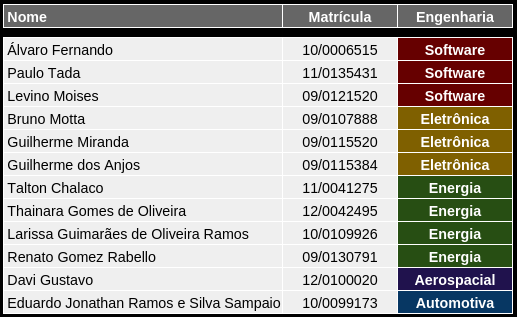
\includegraphics[width=.6\textwidth]{edit/img/equipe.png}
  \caption{Informações sobre a equipe do projeto}
  \label{equipe}
\end{figure}

\subsection{Planejamento da Comunicação}
A estrutura de comunicação do projeto é realizada através de ferramentas colaborativas on-line e reuniões presenciais conforme dispostas pela ementa da disciplina. A disponibilização das comunicações estão dispostas no quadro abaixo, contendo: comunicação, ferramenta, propósito.

\begin{figure}[H]
  \centering
  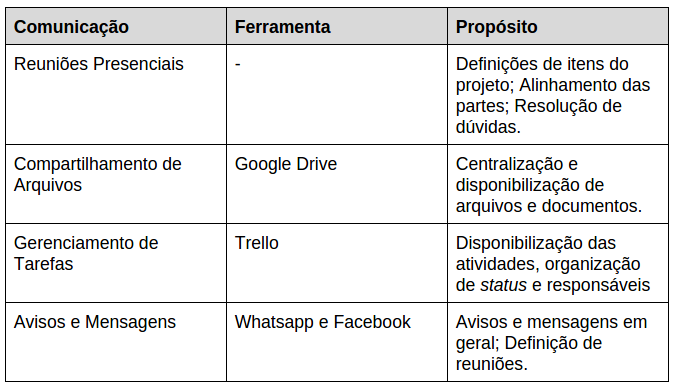
\includegraphics[width=.7\textwidth]{edit/img/comunicacao.png}
  \caption{Definições das comunicações do projeto}
  \label{comunicacao}
\end{figure}
